\newpage
\subsection{Producer}\hfill

%For the main pages put a mockup and describe it in detail.

%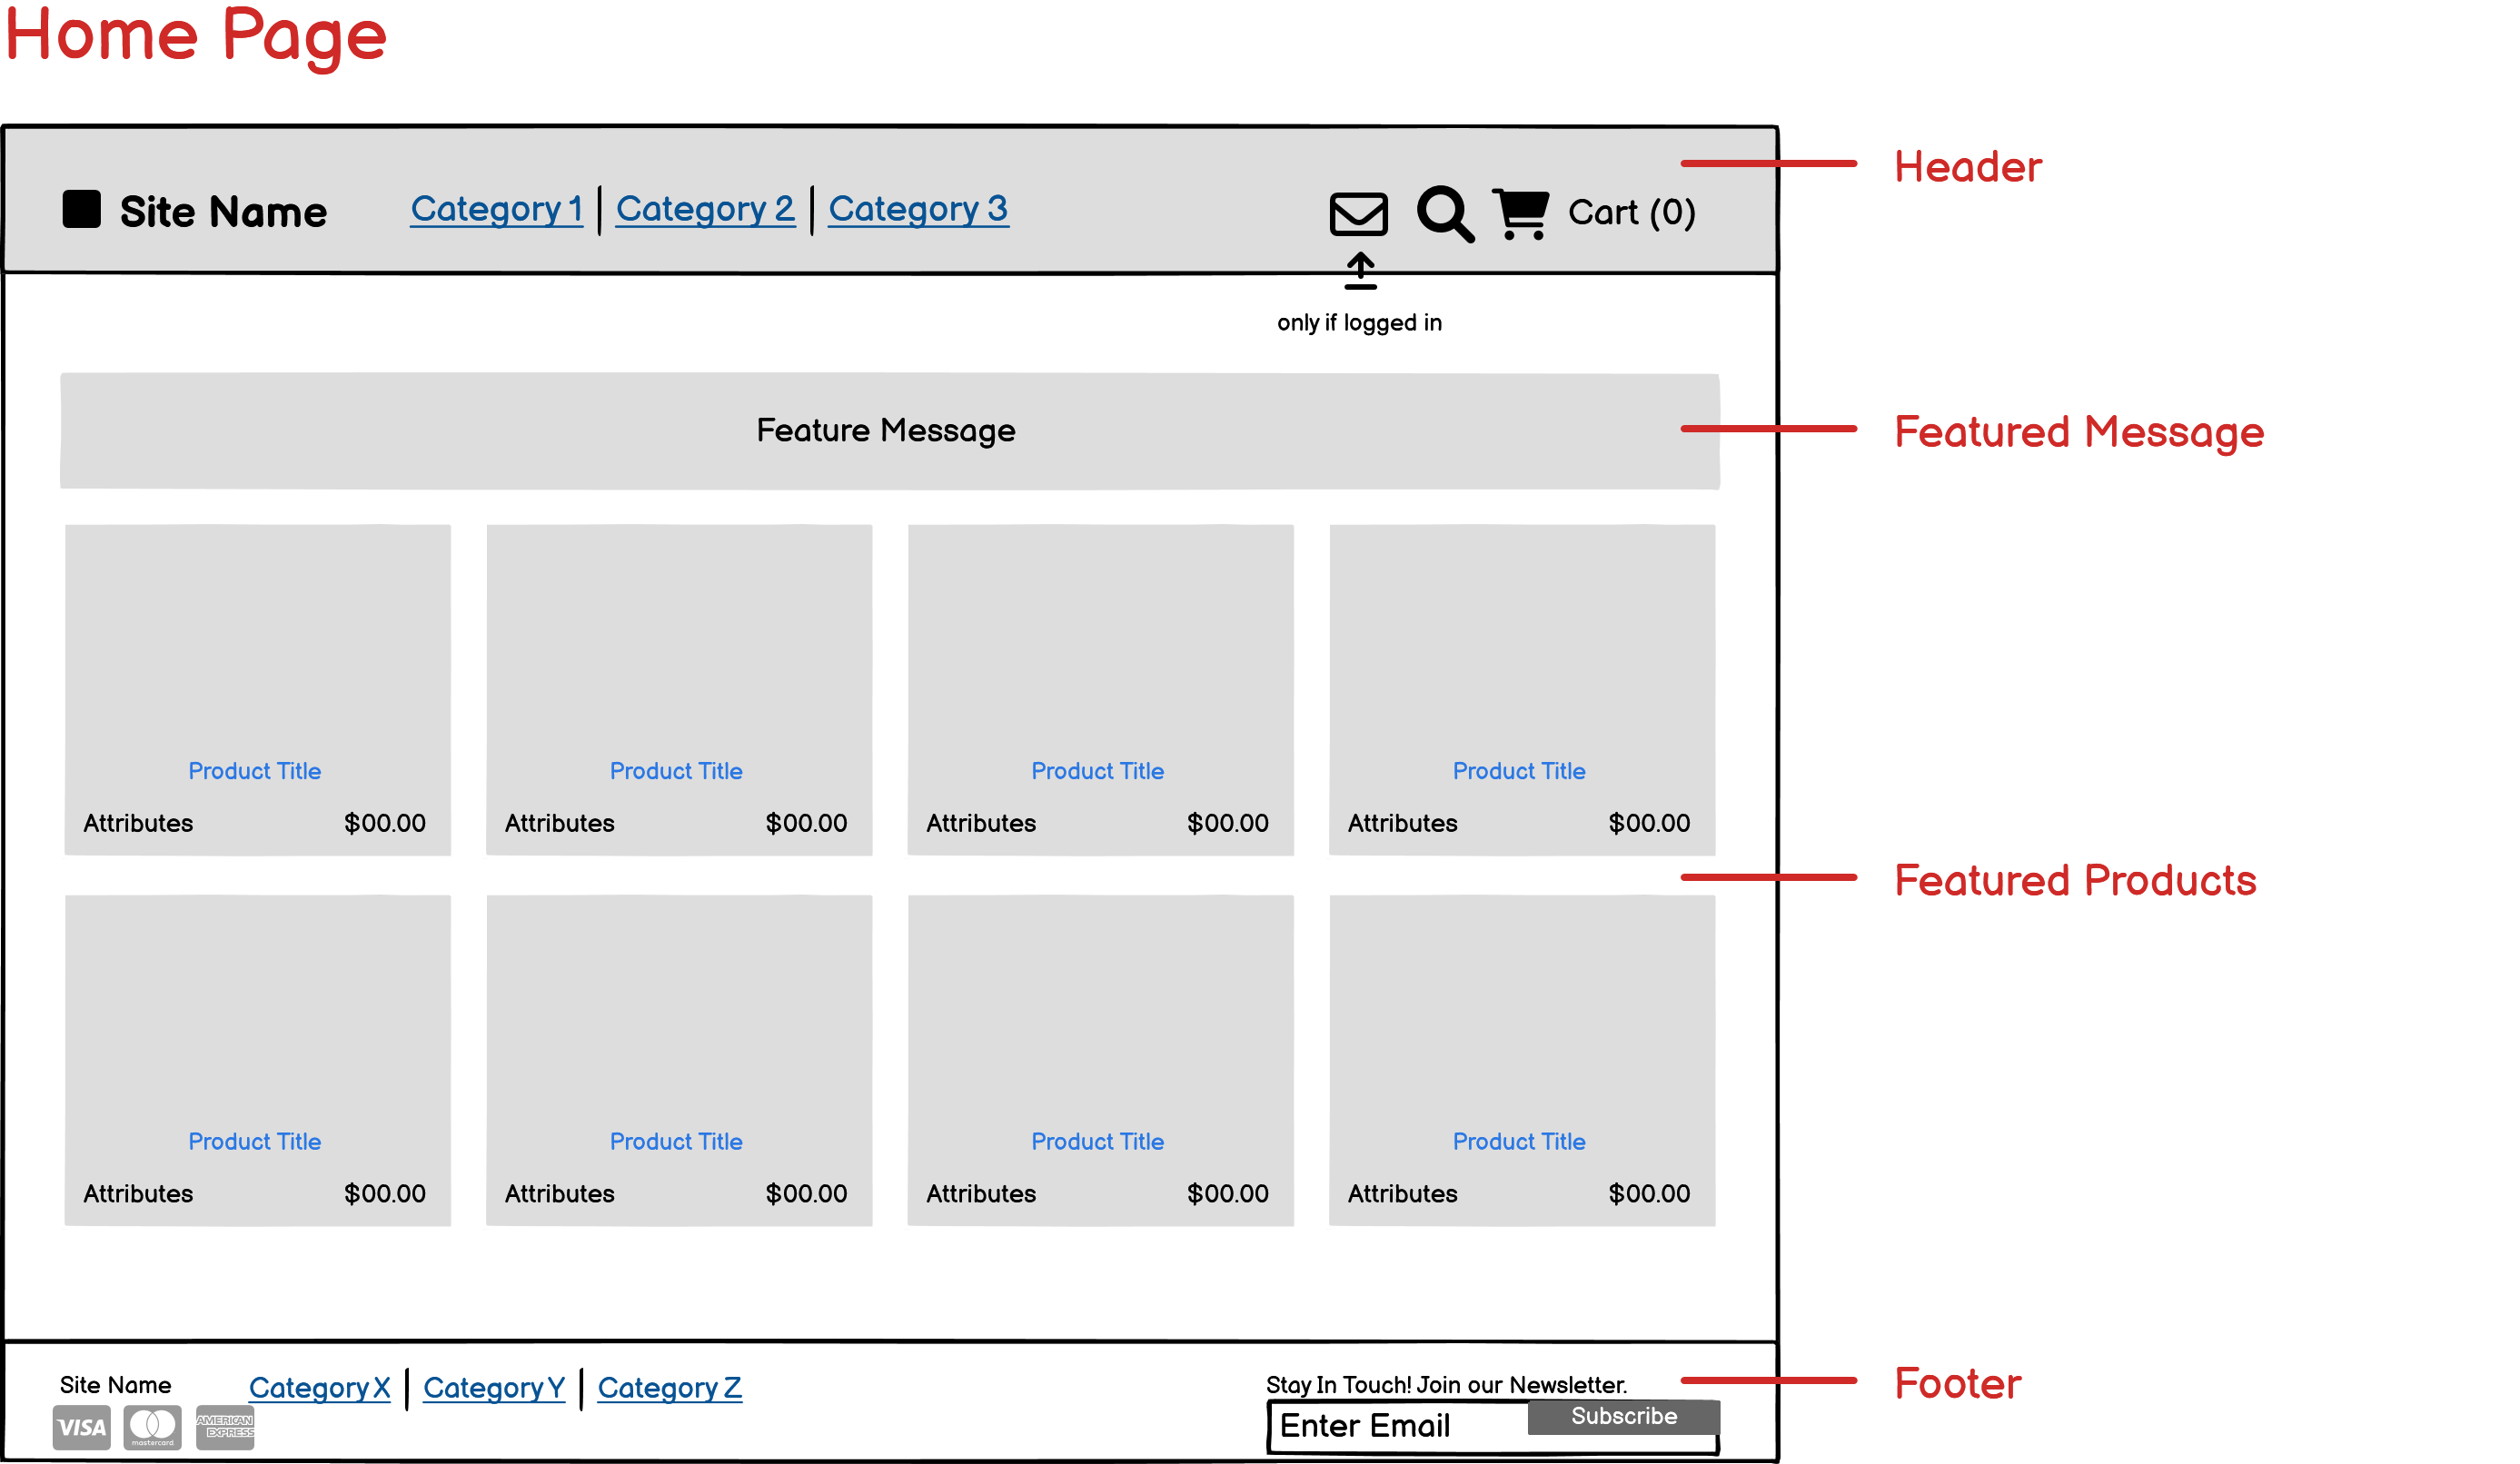
\includegraphics[scale=0.5]{logos/Images/pages/Home Page.png}

\begin{figure}[h]
    \centering
    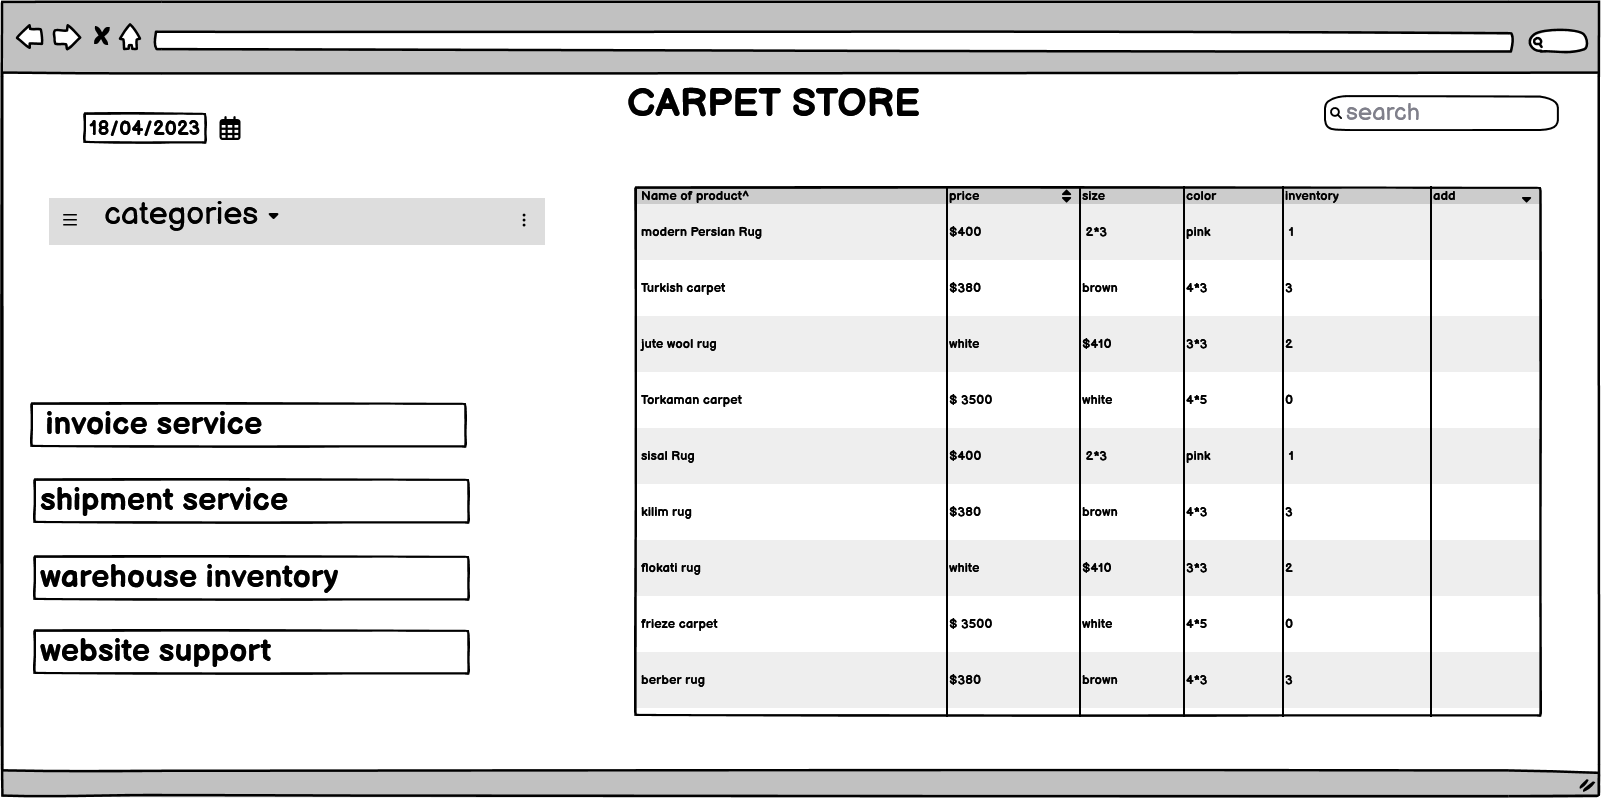
\includegraphics[scale=0.3]{logos/Images/pages/producer 1.png}
    \caption{Producer}
    \label{fig:my_label}
\end{figure}
\hfill \break
On the seller page, the seller has the option to upload products and provide information such as the product name, price, size, color, and inventory. In addition, the seller can select which delivery methods are supported, which tax rates apply, and which payment methods are accepted. The seller can also offer discounts and promotions for products. By clicking the "Add Product" button, the products can be successfully uploaded to the online store. The seller also has the ability to manage inventory and order status, as well as process orders and receive customer feedback.